\chapter{A Simplification Algorithm for Visualizing the Structure of Complex Graphs}
\label{chap:graph_simp}
\section{Introduction} 
Graphs are used to represent and analyze a variety of data sets, from computer network topologies, to cancer cell structures, to research paper citation trends.  Graphs are a useful representation for these types of data, because they naturally provide a clear and distinct way of visualizing the data sets and the interrelationships contained within them.  These data sets are becoming larger and larger, and thus their visual representations are becoming too complex and cluttered.  Graphs frequently have hundreds or thousands of nodes.  Displaying all of these nodes and edges to a user provides no real benefit, since the density and complexity of the graph overwhelms and fills standard displays due to resolution limitations.  Graph simplification provides one way of making these graphs more comprehensible by providing a capability to the user to remove "unimportant" nodes, which then exposes key nodes in the graph and their interconnectivity.  This capability allows the user to interactively examine the structures exposed in simplification; thus enabling the exploration and evaluation of the graph.

In our approach a complex, cluttered graph is progressively thinned by the user until a comprehensible underlying structure in the graph is revealed.  The user may choose from a variety of weighting functions that quantify the importance of the nodes to be removed.  The importance metrics can be based on the topology of the graph or may be provided by an external computational process unrelated to the graph structure itself.  One important feature of the simplification process is that we maintain the connectivity of the graph during pruning.  By default, if the graph is connected at the outset, we ensure that all simplified versions are also connected. The user may also choose not to employ this feature.  For certain types of graphs maintaining connectivity may be important for evaluating node relationships.  In other instances, allowing the graph to split into subgraphs may highlight clusters within the graph.

The simplification process involves two steps.  The first step generates weight values for all nodes in a given graph based on one of our importance metrics.  The second step takes the weighted graph and prunes out less important nodes based on these weight values.  Node removal can be done incrementally, so as to provide different graph resolutions to the user, as well as to ensure that lower importance nodes are removed before higher importance nodes.  The user may also control the connectivity maintenance feature, deciding to preserve the initial graph connectivity during simplification or not.  The simplification algorithm is described in detail in Section \ref{sect:SimpAlg}. Results from applying several of the importance metrics to three types of graphs are presented in Section \ref{sect:Results}.

%-------------------------------------------------------------------------
\section{Related Work}
Related work has been conducted on simplifying graphs, but primarily as a secondary process for manipulating or  matching graphs.  Qiu and Hancock \cite{Qiu-Hancock04,Qiu-Hancock07} develop three graph simplification algorithms.  The first algorithm decomposes a large graph into smaller non-overlapping sub-graphs.  The remaining two carry out simplification based on commute times within the graph.  The algorithms produce a multilayered representation and spanning trees. All three algorithms use their simplified representations to perform matching between the input graphs.

Frishman and Tal \cite{Frishman-Tal07} and Walshaw \cite{Walshaw03} use simplification algorithms to generate simplified graphs for input into their graph layout algorithms.  The simplified graphs are not actually visualized and presented to the user as a way to help them better comprehend the graph data.  Instead, a series of progressively simplified graphs are used to guide the positioning of the nodes in a dense, complex graph.

Additional simplification algorithms have been proposed to assist in robot path planning \cite{Rizzi98}, classifying the topology of surfaces \cite{Ban-Sen03}, speech recognition \cite{LiuHarJohJam03}, and improving the computational complexity and memory requirements of dense graph processing algorithms \cite{KaoOccTen98,suel01compressing,Feder-Motwani95}.

Simplification may also be accomplished through the use of graph clustering.  Girvan and Newman \cite{Girvan-Newman02} define one such clustering-based algorithm for better visualizing the community structure of network graphs.  The kind of graphs that they are targeting with this method are those that would have a naturally occurring community structure.

Rafiei and Curial \cite{Rafiei-Curial05} present another approach to visually simplifying large scale graphs.  They have developed different methods for randomly sampling a graph and using that sampling to construct the visual representation of the graph.  Their general approach is similar to ours in that they are using characteristics of the graphs that frequently occur, but differs in that they reduce their large graphs down to a handful of nodes and then ``grow'' their simplified graph out from those nodes.

Gilbert and Levchenko \cite{Gilbert-Levchenko04} focus on providing metrics for simplifying graphs that represent specific network topologies.  The goal of this work is to simplify and visualize complex network graphs while maintaining their semantic structures.  Although network topologies are certainly reasonable candidates for these visualization techniques, there are other types of graph data that could greatly benefit from simplification techniques for visualization, e.g. the cancer cell graphs produced by Demir et al.~\cite{DemGulYen05} and the citation graphs of Chen~\cite{Chen06}.  These graphs do not consist of the same properties and structures as network topologies, so the metrics of \cite{Gilbert-Levchenko04} may not be valid for these types of graph data.  Our goal is to develop importance metrics that are based on the general topological properties of different types of graphs.  This will allow for the simplification and visualization of any large graph in order for the user to better understand and comprehend its visual representation.

%-------------------------------------------------------------------------
%\cutsectionbefore
\section{Simplification Algorithm}
\label{sect:SimpAlg}

The first step of our simplification algorithm performs an importance metric calculation on the graph, generating a scalar weight value for every node in the graph.  Several importance metrics have been implemented and evaluated, including number of N-ring neighbors, number of shortest paths, node eccentricity, distance to the graph's center node(s), and distance to a leaf node.  It is possible to assign importance values to the graph's nodes based on external factors and calculations not related to the graph's topology.  In this case the calculations of the first step may be skipped, since pruning (the second step) only needs some type of importance value for the nodes, regardless of its origin.

The second step in the algorithm prunes the graph, removing nodes, and associated links, with importance values below a user-specified threshold.  If desired by the user, nodes whose removal would change the graph's connectivity are not pruned from the graph.  Adjusting the threshold value allows the user to control the resolution and complexity of the simplified graph.  The higher the threshold, the more nodes are removed, and the coarser the graph becomes.  The user may choose to remove nodes from the graph incrementally up to the defined threshold value.  Here, a number of pruning steps are applied with successively higher threshold values up to the user defined maximum threshold.


%-------------------------------------------------------------------------
%\cutsubsectionbefore
\subsection{Importance Metrics}
The weight values assigned to the nodes of a graph are computed with different importance metrics.  These metrics are derived from known properties of graph structures.  Currently, none of our metrics are scaled or normalized.  Therefore the range of the resulting values  will vary depending on the metric used, the size of the graph, as well as the topology of the graph.

%-------------------------------------------------------------------------
%\cutsubsubsectionbefore
\subsubsection{Number of N-ring Neighbors}
The first metric is based on the number of N-ring neighbors around a node.  An N-ring neighbor is a node that can be reached in {\em n} unique hops from the original node. When calculating the number of N-ring neighbors where {\em n} is greater than one, the metric may be computed  in two ways.  The metric may count only those neighbors that lie exactly {\em n} hops away from the original node.  The metric may also be cumulative, i.e. it may count all the node that are {\em n} or fewer hops away from the original node.  In this paper we use the first non-cumulative option in calculating the number of N-ring neighbors greater than one.

%\cutsubsubsectionbefore
\subsubsection{Number of Shortest Paths}
The shortest path metric is based on the graph theory principle of betweenness.  A node's betweenness is determined by  how many shortest paths pass through a given node \cite{Wei07}.  This metric finds the shortest path between all nodes $(u,v)$ belonging to graph G using a variation of Dijkstra's shortest path algorithm \cite{Har69}.  For a shortest path between nodes $(u,v)$, each node that belongs to the path has its weight incremented by one. The endpoints of the path do not have their weights incremented. Note that when there are two or more shortest paths of the same length between two nodes one of these is selected at random during the node increment process.
%  With a little bit more coding, we could get around
% this and make the algorithm faster. So let's not admit to it.
% Also, note that each path is counted twice in the algorithm since the process is performed on every node in the graph. For example, the importance value  will be incremented for all nodes along the path from u to v, and along the path from v to u.
This metric is similar to the shortest path based importance metric designed by Gilbert and Levchenko \cite{Gilbert-Levchenko04}.

%-------------------------------------------------------------------------
%\cutsubsubsectionbefore
\subsubsection{Eccentricity}
This metric assigns a node's importance equal to the value of its eccentricity in the graph.  A node's eccentricity is defined as the maximum distance within the set of shortest paths from the node to all other nodes in the graph \cite{Har69}.  Higher values in this metric mean that the given node is a significant distance away from the farthest component in the entire graph, or in other words it is closer to the periphery of the graph than the center.  Therefore the higher the weight value, the less important the node should be.  This is opposite to the definitions of the other metrics.  Thus to be consistent and to lead to proper pruning, the eccentricity importance metric is defined as $eccentricity_i - max(eccentricity)$, where $eccentricity_i$ is the actual eccentricity of a particular node $i$ and $max(eccentricity)$ is computed over all nodes in the graph.

%-------------------------------------------------------------------------
%\cutsubsubsectionbefore
\subsubsection{Shortest Distance to a Center Node}
This metric is a variation on the eccentricity metric mentioned previously.  All nodes with the minimum eccentricity value are defined as center nodes of the graph \cite{Har69}.  These center nodes are important because they have a minimum distance to the farthest limits of the entire graph; thus placing them in the central interior of the graph. Once the center nodes of a graph have been identified, an importance metric can be computed based on the distance to one of the center nodes (there can be more than one).  Nodes with shorter paths are considered more important, because they are closer to the graph's center.  As with the previous metric, this is opposite to the desired importance property. Thus the metric is computed as $distance_i - max(distance)$, where $distance_i$ is the actual shortest distance for a particular node $i$ and $max(distance)$ is computed over all nodes in the graph.



%------------------------------------------------------------------------
%\cutsubsubsectionbefore
\subsubsection{Shortest Distance to a Leaf Node}
This metric calculates the shortest distance from a node to a leaf node in the graph.  It is assumed that the further a node is from a leaf node, the more centrally located within the graph it is, making that node more important.  Ultimately this metric assumes that the input graph will have leaf nodes.  If leaf nodes are not present then this metric cannot be applied during simplification.

%-------------------------------------------------------------------------
%\cutsubsectionbefore
\subsubsection{Network Flow}
Importance metrics do not have to be based solely on quantities derived from the graph's topology.  They can be externally provided by other computations, e.g. network flow calculated for a graph representing a communications network.  A widely-used model for ad-hoc networks is a capacitated directed graph $G(V,E)$ \cite{AMO:flows}, where an edge $(u,v)\in E$ indicates a potential communication link between transmitter $i$ and receiver $j$. The weights $c(u,v)$ on the edges indicate the capacity of the transmission channel, or the maximum amount of information that can be transferred on that channel in a pre-specified amount of time. An important goal in the context of a network is to maximize the amount of information ``flowing'' from a \textit{source} node to a destination (\textit{sink}) node. A good measure of a node's importance given this objective is the outgoing maximum flow from a node on a fully active network.  The maximum flow is computed by solving a flow optimization problem on the graph \cite{Fridman08}.

%------------------------------------------------------------------------
%\cutsubsectionbefore
\subsection{Graph Pruning}

The pruning process visits all nodes and removes those nodes, and their associated edges, with importance values below a user-specified threshold.  Removing a node can cause the graph to fragment.  In order to maintain the basic structure of the graph we do not prune nodes whose removal would split the graph into multiple components and destroy its connectivity.  Gilbert and Levchenko \cite{Gilbert-Levchenko04} do not maintain the connectivity of a graph during pruning.  They reconnect the simplified graph as a post-process.

The connectivity check of the pruning process utilizes our variation on Dijkstra's single source shortest path computation mentioned previously. The candidate node is removed from the graph.  It is then determined if all of the candidate's neighboring nodes are still connected to each other through the graph.  This check is performed by attempting to calculate the shortest path between all pairs of neighboring nodes.  If unable to complete this computation, the graph has been disconnected by the candidate node's removal, and that node is then re-inserted into the graph. 
% Therefore a single iteration of our pruning method will take $O(n^{3})$ worst case when using the connectivity check since in the worst case each node must have its connectivity checked.

The pruning process can be done incrementally. When pruning a weighted graph we use an increment value along with a target threshold value.  The initial threshold is set to 0. The increment is added to this value and the pruning process is performed. The increment is then added to the current threshold and the pruning is performed again on the previously pruned graph. This continues until the current threshold becomes greater than or equal to the target threshold.  Incrementally removing nodes will typically provide better results than a non-incremental removal.  One reason for this is that it tends to remove less important nodes before more important nodes.  When taking large threshold increments it is possible, since nodes are randomly accessed, that a more important node can be processed and pruned before a less important node.  Removing important nodes first may leave less important nodes in a position in which they become impossible to remove due to the connectivity check.  As the increment is decreased the chance of pruning a more important node before a less important node diminishes. Once the increment is equal to the smallest difference between node weight values, incremental pruning effectively produces a removal of nodes in a sorted order, furnishing better results.


%\subsection{Computational Complexity}

%\paragraph*{$N$-Ring Neighbors}
%The time required to compute this metric is, at the worst case, the same as doing a full breadth first search from each node in the graph, which is equal to $O(n * (m+n))$.  The actual running time is dependant on the $N$ valued used which will determine how deep we must go in each breadth first search algorithm.
%\vspace{-5mm}
%\paragraph*{Number of Shortest Paths}
%As mentioned our method of calculating this metric was to uses a variation of Dijkstra's algorithm for computing shortest paths.  Since our algorithm does not involve sotring, it has a running time of $O(n^{3})$.
%\vspace{-5mm}
%\paragraph*{Eccentricity}
%This metric is computed using the all pairs shortest path algorithm from before.  We only need to add a single statement to track the maximum length shortest path from node $i$ to all nodes $j$.  This does not increase the computational complexity.
%\vspace{-5mm}
%\paragraph*{Distance to a Center Node}
%This metric requires two parts, first calculating the eccentricity values and then calculating the shortest path from all nodes to the defined center nodes.  This first part, as described above, makes use of the all pairs shortest paths algorithm.  We then perform this algorithm again but for each source we stop once we have found a center node.  The worst case running time is simply $2* O(n^{3})$.
%\vspace{-5mm}
%\paragraph*{Distance to a Leaf Node}
%The method again uses the all pair shortest path algorithm where for each source we stop once we find a leaf node.  The worst case running time is still the same as for all pairs shortest path.

%-------------------------------------------------------------------------
%\cutsectionbefore
\section{Test Data}
\label{sect:Data}
Our graph simplification algorithm and all of its metrics have been applied to a number of graphs.  The algorithm has been tested and evaluated on three different types of graphs. The first graph was automatically generated using the  Inet tool \cite{Winik-Jamin02}, a power-law-based graph generator that creates graphs representing internet topologies.  The Inet graph we used in our testing had 4500 vertices and 15308 edges.

The second graph was generated from data produced by the citation trends research of Chen \cite{Chen06}.  Each node of the citation graph is a research paper and every edge represents a citation of that paper.  Originally this was a directed graph, but since most of our metrics do not utilize the direction associated with an edge, we assume that the citation graph is undirected.  Although we lose some of the graph's information, it still provides a unique real-world graph structure for evaluation.  This citation graph had 1025 vertices and 15430 edges.

We also include a graph generated from the OMAN  ad-hoc network simulator, a simulation system developed at Drexel University.  The nodes of this graph are pre-weighted using the OMAN-computed flow metrics discussed previously.  We imported the graph along with its weight values and processed it with our pruning mechanism to demonstrate that the pruning operation is independent from our importance metrics calculations and is capable of handling different types of graphs.

In order to better visualize these graphs, they have each been pre-processed with the neato graph layout tool of Graphviz \cite{Graphviz}.  This applies a spring model layout to our graphs prior to applying our simplification algorithm.

%-------------------------------------------------------------------------
%\cutsectionbefore
\section{Metric Performance Criteria}
\label{sect:metric_criteria}

Once the various importance metrics were implemented and applied to the first two graphs, general properties of their resulting values were observed.  In evaluating how each metric performed we first define what we believe makes an effective importance metric in terms of using it to simplify the graph
for visualization.

%TODO: review the definition of a good metric, try and flush it out some more.
First, a metric should provide a wide range of weight values across the nodes.  A wider range allows for finer control of the resolution of the simplified graph. This property can be evaluated by the ratio of the range of weight values to the number of nodes in the graph. An example is metric $A$ generates weights in the range of 0 to 400 on a graph $G$ with 1000 nodes.  The weight-range-to-node-count ratio would then be $400/1000 = 0.4:1$.  This provides a consistent way to compare each metric's characteristics across a single graph.  We have captured this data for all of our metrics and test graphs in Table~\ref{tbl:weight_ratio}.

An effective metric should also create a even distribution of these weight values across the entire range.  An even distribution will allow for a more controlled simplification of the graph as the user increases the threshold value.  This allows the user to control the resolution of the resulting
simplified graph.  This distribution can be measured by observing the rate at which nodes are removed from the graph while simplifying over the range of weight values.  


\section{Results}
\label{sect:Results}
Using the metric performance criteria defined in Section~\ref{sect:metric_criteria}, we offer an evaluation of each of our weighting metrics when applied to our test data.  The distribution of the weight values across the range of weights is illustrated in Figure~\ref{fig:node_drop_off}.  The data in these graphs was generated by taking the range of the weight values of each metric on a given graph and dividing it into equal increments.  Data in these graphs was generated by taking the range of the weight values of each metric on a given graph and dividing it into 18 equal increments.  The simplification process was then run at each increment, and the number of nodes remaining after the simplification was then recorded.

\begin{figure*}[htp]
\begin{center}
 \scalebox
 {0.80} % h_length
 {
 \includegraphics{images/citation_graph_node_drop_off.eps}
 }
 
 \scalebox
 {0.80}
 {
 \includegraphics{images/inet4500_node_drop_off.eps}
 }
\end{center}
\caption{\label{fig:node_drop_off}
Two graphs showing the node drop off rate of each metric against the Citation graph \cite{Chen06} (top) and an Inet graph (bottom).  The min and max weight were determined for each metric on the particular graph.  This range was then divided into equal increments and the simplification process was run at each increment with the threshold value being equal to each increment.  The number of nodes remaining at each increment was recorded.
}
\end{figure*}


\begin{table*}
\begin{center}
\begin{tabular}{|l|l|l|l|l|}
\hline
 & \multicolumn{2}{|c|}{Citation Graph} & \multicolumn{2}{|c|}{Inet4500} \\
\hline
Metric & Weight Range & Ratio & Weight Range & Ratio \\
\hline
1-Ring& 1 to 75 & 0.0721 & 1 to 942 & 0.2093 \\
num-short & 2 to 380 & 0.3687 & 2 to 3585 & 0.79667 \\
3-Ring & 3 to 763 & 0.7414  & 3 to 4432 & 0.9842 \\
Shortest Path & 0 to 85284 & 83.2039 & 0 to 12926842 & 2872.6315 \\
Dist to Leaf & 0 to 7 & 0.0068 & 0 to 4 & 0.0008 \\
Dist to Center & 1 to 10 & 0.0087 & 1 to 6 & 0.0011 \\
Eccentricity & 9 to 17 & 0.0087 & 5 to 9 & 0.0008 \\
\hline
\end{tabular}
\caption{This table lists the Weight Range to \# of Nodes ratios for each metric and each graph they were run against.}
\label{tbl:weight_ratio}
\end{center}
\end{table*}



%TODO: Relate the evaluation of each metric to the criteria of a good metric.
\paragraph*{N-ring Neighbors.}
For N-Ring neighbors we implemented three variations of the metric.  We tested one, two, and three ring neighbors as metrics.  Overall the N-ring neighbors metric generates reasonable weight ranges.  A comparison of the weight-range-to-node-count ratios for each of the three variations can be seen in
Table \ref{tbl:weight_ratio}.  We can see that as we increase $N$, the ratios approach $1:1$.  These metrics of course are dependent on the connectivity of the original graph; but since we are primarily focusing on large complex graphs, these metrics provide good ranges for these types of graphs.

The node drop off rates for these metrics also showed a similar relationship as $N$ was increased.  In Figure~\ref{fig:node_drop_off} the three N-Ring metrics start off with a quick drop off at the beginning of the weight range and as $N$ increases, the node drop off rate becomes approximately linear.  This indicates that the distribution of weight values across the entire range becomes more evenly spread out as $N$ is increased.

Figures~\ref{fig:Inet-2-ring} show an example of the visual result generated by applying the 2-ring neighbors metric on the Inet graph.  Figures~\ref{fig:cite-3-ring} show the result of applying the 3-ring neighbors metric to the Citation graph.

\begin{figure}[ht]
\centering
\subfigure[]{
	\includegraphics[height=0.33\linewidth,width=0.33\linewidth]{images/inet4500/m2/inet4500_m[2]_t[300].ps}
	\label{fig:Inet-2-ring-300}
}
\subfigure[]{
	\includegraphics[height=0.33\linewidth,width=0.33\linewidth]{images/inet4500/m2/inet4500_m[2]_t[700].ps}
	\label{fig:Inet-2-ring-700}
}
\subfigure[]{
	\includegraphics[height=0.33\linewidth,width=0.33\linewidth]{images/inet4500/m2/inet4500_m[2]_t[1200].ps}
	\label{fig:Inet-2-ring-1200}
}
\subfigure[]{
	\includegraphics[height=0.33\linewidth,width=0.33\linewidth]{images/inet4500/m2/inet4500_m[2]_t[1800].ps}
	\label{fig:Inet-2-ring-1800}
}
\caption{Inet graph with 4500 Nodes: 2-Ring Neighbors metric with threshold values \subref{fig:Inet-2-ring-300}300, \subref{fig:Inet-2-ring-700}700, \subref{fig:Inet-2-ring-1200}1200, \subref{fig:Inet-2-ring-1800}1800.}
\label{fig:Inet-2-ring}

\end{figure}

\begin{figure}[ht]
\centering
\subfigure[]{
	\includegraphics[height=0.33\linewidth,width=0.33\linewidth]{images/citation_graph/m3/citation_graph_m[3]_t[360].ps}
	\label{fig:cite-3-ring-360}
}
\subfigure[]{
	\includegraphics[height=0.33\linewidth,width=0.33\linewidth]{images/citation_graph/m3/citation_graph_m[3]_t[504].ps}
	\label{fig:cite-3-ring-504}
}
\subfigure[]{
	\includegraphics[height=0.33\linewidth,width=0.33\linewidth]{images/citation_graph/m3/citation_graph_m[3]_t[576].ps}
	\label{fig:cite-3-ring-576}
}
\subfigure[]{
	\includegraphics[height=0.33\linewidth,width=0.33\linewidth]{images/citation_graph/m3/citation_graph_m[3]_t[648].ps}
	\label{fig:cite-3-ring-648}
}
\caption{Citation Graph with 1025 Nodes: 3-Ring Neighbors metric with threshold values \subref{fig:cite-3-ring-360}360, \subref{fig:cite-3-ring-504}504, \subref{fig:cite-3-ring-576}576, \subref{fig:cite-3-ring-648}648.}
\label{fig:cite-3-ring}

\end{figure}

Overall all the properties exhibited by the N-Ring neighbors metrics define them as effective  metrics.  The range of weights across the nodes and the distribution of those weight values are both in line with our definition of a good metric.

%-------------------------------------------------------------------------
\paragraph*{Number of Shortest Paths.}
The Shortest Path metric calculates very high weight values for frequently visited nodes in the center of the graph.  There is a large number of paths through these central nodes since they allow the outer nodes to connect most directly with each other.  This can be seen in its node drop off rate curve in Figure~\ref{fig:node_drop_off}.  Initially there is a very quick drop off of nodes. These removed nodes would exist more towards the periphery of the graph.  This initial drop off tends to eliminate approximately half of the nodes in the graph within a few pruning steps.  Once these nodes are removed the curve becomes much more linear in its rate of decent.  This shows that the distribution of weights is very biased towards the lower end of the range.

The ratio of weight range to number of nodes on the other hand is quite large.  For the citation graph the Shortest Path metric generated a ratio of $83.2:1$ and for the inet graph a ratio of $2872.6:1$ was generated.  With such large weight-range-to-node-count ratios the difference between simplifying with two distinct threshold values may be only one or two nodes.

Figures~\ref{fig:Inet-num-short} show an example of the visual result generated by applying the number of shortest paths metric on the Inet graph.  Figures~\ref{fig:cite-num-short} show the result of applying this metric to the Citation graph.

\begin{figure}[ht]
\centering
\subfigure[]{
	\includegraphics[height=0.33\linewidth,width=0.33\linewidth]{images/inet4500/m4/inet4500_m[4]_t[1000].ps}
	\label{fig:Inet-num-short-1000}
}
\subfigure[]{
	\includegraphics[height=0.33\linewidth,width=0.33\linewidth]{images/inet4500/m4/inet4500_m[4]_t[40000].ps}
	\label{fig:Inet-num-short-40000}
}
\subfigure[]{
	\includegraphics[height=0.33\linewidth,width=0.33\linewidth]{images/inet4500/m4/inet4500_m[4]_t[100000].ps}
	\label{fig:Inet-num-short-100000}
}
\subfigure[]{
	\includegraphics[height=0.33\linewidth,width=0.33\linewidth]{images/inet4500/m4/inet4500_m[4]_t[645000].ps}
	\label{fig:Inet-num-short-645000}
}
\caption{Inet graph with 4500 Nodes: Shortest Paths metric with threshold values \subref{fig:Inet-num-short-1000}1000, \subref{fig:Inet-num-short-40000}40000, \subref{fig:Inet-num-short-100000}100000, \subref{fig:Inet-num-short-645000}645000.}
\label{fig:Inet-num-short}

\end{figure}

\begin{figure}[ht]
\centering
\subfigure[]{
	\includegraphics[height=0.33\linewidth,width=0.33\linewidth]{images/citation_graph/m4/citation_graph_m[4]_t[1404].ps}
	\label{fig:cite-num-short-1404}
}
\subfigure[]{
	\includegraphics[height=0.33\linewidth,width=0.33\linewidth]{images/citation_graph/m4/citation_graph_m[4]_t[4212].ps}
	\label{fig:cite-num-short-4212}
}
\subfigure[]{
	\includegraphics[height=0.33\linewidth,width=0.33\linewidth]{images/citation_graph/m4/citation_graph_m[4]_t[28828].ps}
	\label{fig:cite-num-short-28828}
}
\subfigure[]{
	\includegraphics[height=0.33\linewidth,width=0.33\linewidth]{images/citation_graph/m4/citation_graph_m[4]_t[48828].ps}
	\label{fig:cite-num-short-48828}
}
\caption{Citation Graph with 1025 Nodes: Shortest Paths metric with threshold values \subref{fig:cite-num-short-1404}1404, \subref{fig:cite-num-short-4212}4212, \subref{fig:cite-num-short-28828}28828, \subref{fig:cite-num-short-48828}48828.}
\label{fig:cite-num-short}

\end{figure}

Overall the metric does not fit very well into our definition of an effective metric.  The weight distribution tends to be heavily biased to the lower end of what is typically a very large range of weight values.  Such a large range of weight values actually gives too much granularity between each distinct threshold value in the higher weighted nodes.  The removal of one or two nodes rarely makes any distinguishable visible difference in the graphs.  This metric could be made more effective by scaling or normalizing the generated weight values.  Doing this should even out the distribution and contract the overly large range of weight values.

%-------------------------------------------------------------------------
\paragraph*{Eccentricity.}
The Eccentricity metric provides some interesting results.  This metric depends on the underlying connectivity of the original graph.  We can observe this by looking at the weight-range-to-node-count ratios.  For both graphs this ratio we extremely low, $0.00088:1$ for the inet graph and $0.00878:1$ for the citation graph.  The actual range of weight values for the inet graph was from 0 to 4.  This means that the longest shortest path within this graph is length 4.  This implies one of two things, that the graph is very well connected or it reveals a radial graph structure that flows into a few central nodes.

Figures~\ref{fig:Inet-ecc} show an example of the visual result generated by applying the Eccentricity metric on the Inet graph.  Figures~\ref{fig:cite-ecc} show the result of applying this metric to the Citation graph.

\begin{figure}[ht]
\centering
\subfigure[]{
	\includegraphics[height=0.33\linewidth,width=0.33\linewidth]{images/inet4500/m11/inet4500_m[11]_t[7].ps}
	\label{fig:Inet-ecc-7}
}
\subfigure[]{
	\includegraphics[height=0.33\linewidth,width=0.33\linewidth]{images/inet4500/m11/inet4500_m[11]_t[8].ps}
	\label{fig:Inet-ecc-8}
}
\subfigure[]{
	\includegraphics[height=0.33\linewidth,width=0.33\linewidth]{images/inet4500/m11/inet4500_m[11]_t[10].ps}
	\label{fig:Inet-ecc-10}
}
\subfigure[]{
	\includegraphics[height=0.33\linewidth,width=0.33\linewidth]{images/inet4500/m11/inet4500_m[11]_t[12].ps}
	\label{fig:Inet-ecc-12}
}
\caption{Inet graph with 4500 Nodes: Eccentricity metric with threshold values \subref{fig:Inet-ecc-7}7, \subref{fig:Inet-ecc-8}8, \subref{fig:Inet-ecc-10}10, \subref{fig:Inet-ecc-12}12.}
\label{fig:Inet-ecc}

\end{figure}

\begin{figure}[ht]
\centering
\subfigure[]{
	\includegraphics[height=0.33\linewidth,width=0.33\linewidth]{images/citation_graph/m11/citation_graph_m[11]_t[10].ps}
	\label{fig:cite-ecc-10}
}
\subfigure[]{
	\includegraphics[height=0.33\linewidth,width=0.33\linewidth]{images/citation_graph/m11/citation_graph_m[11]_t[13].ps}
	\label{fig:cite-ecc-13}
}
\subfigure[]{
	\includegraphics[height=0.33\linewidth,width=0.33\linewidth]{images/citation_graph/m11/citation_graph_m[11]_t[15].ps}
	\label{fig:cite-ecc-15}
}
\subfigure[]{
	\includegraphics[height=0.33\linewidth,width=0.33\linewidth]{images/citation_graph/m11/citation_graph_m[11]_t[19].ps}
	\label{fig:cite-ecc-19}
}
\caption{Citation Graph with 1025 Nodes: Eccentricity metric with threshold values \subref{fig:cite-ecc-10}10, \subref{fig:cite-ecc-13}13, \subref{fig:cite-ecc-15}15, \subref{fig:cite-ecc-19}19.}
\label{fig:cite-ecc}

\end{figure}

The distribution of these weight values is also highly dependent on the underlying structure of the graph.  We see that for the citation graph this metric provides a relatively even drop off rate while the Inet graph has a very sharp drop off over the middle weight values in its range.

%-------------------------------------------------------------------------
\paragraph*{Shortest Distance to Center Node.}
Since this metric is based on the graph's eccentricity, it displays many of the same properties as the Eccentricity metric.  It maintains very low weight-range-to-node-count ratios, $0.0011:1$ and $0.0087:1$ for the Inet and citation graphs respectively, and the distribution is again dependent on the structure of the graph being processed.

Figures~\ref{fig:Inet-center} show an example of the visual result generated by applying the Shortest Distance to Center Node metric on the Inet graph.  Figures~\ref{fig:cite-center} show the result of applying this metric to the Citation graph.

\begin{figure}[ht]
\centering
\subfigure[]{
	\includegraphics[height=0.33\linewidth,width=0.33\linewidth]{images/inet4500/m10/inet4500_m[10]_t[3].ps}
	\label{fig:Inet-center-3}
}
\subfigure[]{
	\includegraphics[height=0.33\linewidth,width=0.33\linewidth]{images/inet4500/m10/inet4500_m[10]_t[4].ps}
	\label{fig:Inet-center-4}
}
\subfigure[]{
	\includegraphics[height=0.33\linewidth,width=0.33\linewidth]{images/inet4500/m10/inet4500_m[10]_t[5].ps}
	\label{fig:Inet-center-5}
}
\subfigure[]{
	\includegraphics[height=0.33\linewidth,width=0.33\linewidth]{images/inet4500/m10/inet4500_m[10]_t[6].ps}
	\label{fig:Inet-center-6}
}
\caption{Inet graph with 4500 Nodes: Shortest Distance to a Center Node metric with threshold values \subref{fig:Inet-center-3}3, \subref{fig:Inet-center-4}4, \subref{fig:Inet-center-5}5, \subref{fig:Inet-center-6}6.}
\label{fig:Inet-center}

\end{figure}

\begin{figure}[ht]
\centering
\subfigure[]{
	\includegraphics[height=0.33\linewidth,width=0.33\linewidth]{images/citation_graph/m10/citation_graph_m[10]_t[5].ps}
	\label{fig:cite-center-5}
}
\subfigure[]{
	\includegraphics[height=0.33\linewidth,width=0.33\linewidth]{images/citation_graph/m10/citation_graph_m[10]_t[6].ps}
	\label{fig:cite-center-6}
}
\subfigure[]{
	\includegraphics[height=0.33\linewidth,width=0.33\linewidth]{images/citation_graph/m10/citation_graph_m[10]_t[7].ps}
	\label{fig:cite-center-7}
}
\subfigure[]{
	\includegraphics[height=0.33\linewidth,width=0.33\linewidth]{images/citation_graph/m10/citation_graph_m[10]_t[8].ps}
	\label{fig:cite-center-8}
}
\caption{Citation Graph with 1025 Nodes: Shortest Distance to a Center Node metric with threshold values \subref{fig:cite-center-5}5, \subref{fig:cite-center-6}6, \subref{fig:cite-center-7}7, \subref{fig:cite-center-8}8.}
\label{fig:cite-center}

\end{figure}

While this metric and Eccentricity have some similarities, there are some differences in the resulting weights.  In the Eccentricity metric a node relatively close to a center node may have a lower metric value because of the variety of paths available to reach all other nodes.  While that same node may have a high Center Node metric value simply because it is near a center node.  In a network analogy a given node may not need to reach the edges of the network directly.  Instead it connects to a more centrally located node which handles the distribution.  In this case the Distance to Center metric will capture this property.

%-------------------------------------------------------------------------
\paragraph*{Shortest Path to Leaf Node.}
The Shortest Path to a Leaf Node metric is another that is highly dependent on the topological structure of the original graph.  Firstly, it assumes that the given graph does contain leaf nodes.  If it does not then this metric cannot be computed.  In relating this metric to our standards for an effective metric, this one is a bit weak.  Its weight-range-to-node-count ratios are fairly small.  The citation graph's ratio was $0.0068:1$ while the inet graph's was $0.00088:1$.  These values are about the same as the Eccentricity and Distance to Center Node metrics.  The node drop off rates follow a trend similar to that of the Eccentricity and Distance to Center Node metrics as seen in Figure~\ref{fig:node_drop_off}.

Figures~\ref{fig:Inet-leaf} show an example of the visual result generated by applying the Shortest Distance to Center Node metric on the Inet graph.  Figures~\ref{fig:cite-leaf} show the result of applying this metric to the Citation graph.

\begin{figure}[ht]
\centering
\subfigure[]{
	\includegraphics[height=0.33\linewidth,width=0.33\linewidth]{images/inet4500/m9/inet4500_m[9]_t[3].ps}
	\label{fig:Inet-leaf-3}
}
\subfigure[]{
	\includegraphics[height=0.33\linewidth,width=0.33\linewidth]{images/inet4500/m9/inet4500_m[9]_t[5].ps}
	\label{fig:Inet-leaf-5}
}
\subfigure[]{
	\includegraphics[height=0.33\linewidth,width=0.33\linewidth]{images/inet4500/m9/inet4500_m[9]_t[6].ps}
	\label{fig:Inet-leaf-6}
}
\subfigure[]{
	\includegraphics[height=0.33\linewidth,width=0.33\linewidth]{images/inet4500/m9/inet4500_m[9]_t[7].ps}
	\label{fig:Inet-leaf-7}
}
\caption{Inet graph with 4500 Nodes: Shortest Path to a Leaf Node metric with threshold values \subref{fig:Inet-leaf-3}3, \subref{fig:Inet-leaf-5}5, \subref{fig:Inet-leaf-6}6, \subref{fig:Inet-leaf-7}7.}
\label{fig:Inet-leaf}

\end{figure}

\begin{figure}[ht]
\centering
\subfigure[]{
	\includegraphics[height=0.33\linewidth,width=0.33\linewidth]{images/citation_graph/m9/citation_graph_m[9]_t[2].ps}
	\label{fig:cite-leaf-2}
}
\subfigure[]{
	\includegraphics[height=0.33\linewidth,width=0.33\linewidth]{images/citation_graph/m9/citation_graph_m[9]_t[5].ps}
	\label{fig:cite-leaf-5}
}
\subfigure[]{
	\includegraphics[height=0.33\linewidth,width=0.33\linewidth]{images/citation_graph/m9/citation_graph_m[9]_t[6].ps}
	\label{fig:cite-leaf-6}
}
\subfigure[]{
	\includegraphics[height=0.33\linewidth,width=0.33\linewidth]{images/citation_graph/m9/citation_graph_m[9]_t[9].ps}
	\label{fig:cite-leaf-9}
}
\caption{Citation Graph with 1025 Nodes: Shortest Path to a Leaf Node metric with threshold values \subref{fig:cite-leaf-2}2, \subref{fig:cite-leaf-5}5, \subref{fig:cite-leaf-6}6, \subref{fig:cite-leaf-9}9.}
\label{fig:cite-leaf}

\end{figure}

Overall this metric is designed to give a good measure of how well connected the leaf nodes of a graph may be.  It can also offer insight into how well the non-leaf nodes are connected amongst each other. If the metric's values tend to be high, then the non-leaf nodes are not very well-connected and need to follow longer paths to get to the periphery of the graph.

%-------------------------------------------------------------------------
\paragraph*{Network Flow}
The computation of the Network Flow metric is one based on criteria other than the topology of the given graph.  Therefore our performance criteria does not hold when evaluating this metric.  We can see the results of applying the pruning algorithm to the flow graph shown in Figures~\ref{fig:flow}.  These images present a steady thinning of the graph, while maintaining its connectivity. The T=6000 graph shows the drop out of all the low flow nodes in the network. The T=18000 graph continues to simplify the display of the network so we can start to see a more defined structure to the higher flowing nodes.  The transition from the T=18000 graph to the T=50000 graph then reveals those nodes that have significant flow coming out of them, marking them as nodes which are important for flowing lots of information through the network.

\begin{figure}[ht]
\centering
\subfigure[]{
	\includegraphics[height=0.33\linewidth,width=0.33\linewidth]{images/oman_v1000/oman_v1000_t[0].ps}
	\label{fig:flow-0}
}
\subfigure[]{
	\includegraphics[height=0.33\linewidth,width=0.33\linewidth]{images/oman_v1000/oman_v1000_t[6000].ps}
	\label{fig:flow-6000}
}
\subfigure[]{
	\includegraphics[height=0.33\linewidth,width=0.33\linewidth]{images/oman_v1000/oman_v1000_t[18000].ps}
	\label{fig:flow-18000}
}
\subfigure[]{
	\includegraphics[height=0.33\linewidth,width=0.33\linewidth]{images/oman_v1000/oman_v1000_t[50000].ps}
	\label{fig:flow-50000}
}
\caption{Inet graph with 4500 Nodes: Shortest Path to a Leaf Node metric with threshold values \subref{fig:flow-0}0, \subref{fig:flow-6000}6000, \subref{fig:flow-18000}18000, \subref{fig:flow-50000}50000.}
\label{fig:flow}

\end{figure}

%-------------------------------------------------------------------------
\paragraph*{Algorithm Run-time Performance}
The computation time needed to perform simplification is not significant. Each graph simplification requires about a second to a few tens of seconds (with a rare simplification using the Number of Shortest Paths metric needing about a CPU-minute) to compute, with most of the graph processing requiring only a few CPU-seconds on an Intel Dual Core 1.73 GHz processor. These times were to both compute the given metric and prune the graph incrementally while preserving connectivity.  Times varied slightly based on the metric calculated, graph size, and threshold and increment values.


%-------------------------------------------------------------------------
%\cutsectionbefore
\section{Conclusion}
Complex graphs, ones containing thousands of nodes of high degree, are difficult to visualize. Displaying all of the nodes and edges of these graphs can create an incomprehensible cluttered output.  We have presented a simplification algorithm that may be applied to a complex graph in order to produce a controlled thinning of the graph. The simplification of the graph provides an approach to visualizing and examining some of the underlying structures of the graph by displaying the most important nodes, where importance may be based on the topology of the graph or external factors.  The simplification algorithm consists of two steps, calculation of importance metrics and pruning.  We have described several weighting functions and have presented the simplified graphs produced by applying them.  Future work includes developing additional importance metrics, as well as testing and evaluating our approach on other types of graphs.
